%%%%%%%%%%%%%%%%%%%%%%%%%%%%%%%%%%%%%%%%%
% Beamer Presentation
% LaTeX Template
% Version 1.0 (10/11/12)
%
% This template has been downloaded from:
% http://www.LaTeXTemplates.com
%
% License:
% CC BY-NC-SA 3.0 (http://creativecommons.org/licenses/by-nc-sa/3.0/)
%
%%%%%%%%%%%%%%%%%%%%%%%%%%%%%%%%%%%%%%%%%

%----------------------------------------------------------------------------------------
%    PACKAGES AND THEMES
%----------------------------------------------------------------------------------------

\documentclass{beamer}
\usepackage{animate}
\usepackage{float}
\usepackage{bm}
\usepackage{mathtools}
\usepackage{extarrows}

\newcommand{\ChoL}{\mathsf{L}}
\newcommand{\bx}{\mathbf{x}}
\newcommand{\ii}{\mathrm{i}}
\newcommand{\bxi}{\bm{\xi}}
\newcommand{\bmu}{\bm{\mu}}
\newcommand{\bb}{\mathbf{b}}
\newcommand{\bA}{\mathbf{A}}
\newcommand{\bJ}{\mathbf{J}}
\newcommand{\bB}{\mathbf{B}}
\newcommand{\bM}{\mathbf{M}}

\newcommand{\by}{\mathbf{y}}
\newcommand{\bw}{\mathbf{w}}

\newcommand{\bX}{\mathbf{X}}
\newcommand{\bY}{\mathbf{Y}}
\newcommand{\bs}{\mathbf{s}}
\newcommand{\sign}{\mathrm{sign}}
\newcommand{\bt}[0]{\bm{\theta}}
\newcommand{\bc}{\mathbf{c}}
\newcommand{\bzero}{\mathbf{0}}
\renewcommand{\bf}{\mathbf{f}}
\newcommand{\bu}{\mathbf{u}}
\newcommand{\bv}[0]{\mathbf{v}}

\mode<presentation> {

% The Beamer class comes with a number of default slide themes
% which change the colors and layouts of slides. Below this is a list
% of all the themes, uncomment each in turn to see what they look like.

%\usetheme{default}
%\usetheme{AnnArbor}
%\usetheme{Antibes}
%\usetheme{Bergen}
%\usetheme{Berkeley}
%\usetheme{Berlin}
%\usetheme{Boadilla}
%\usetheme{CambridgeUS}
%\usetheme{Copenhagen}
%\usetheme{Darmstadt}
%\usetheme{Dresden}
%\usetheme{Frankfurt}
%\usetheme{Goettingen}
%\usetheme{Hannover}
%\usetheme{Ilmenau}
%\usetheme{JuanLesPins}
%\usetheme{Luebeck}
\usetheme{Madrid}
%\usetheme{Malmoe}
%\usetheme{Marburg}
%\usetheme{Montpellier}
%\usetheme{PaloAlto}
%\usetheme{Pittsburgh}
%\usetheme{Rochester}
%\usetheme{Singapore}
%\usetheme{Szeged}
%\usetheme{Warsaw}


% As well as themes, the Beamer class has a number of color themes
% for any slide theme. Uncomment each of these in turn to see how it
% changes the colors of your current slide theme.

%\usecolortheme{albatross}
\usecolortheme{beaver}
%\usecolortheme{beetle}
%\usecolortheme{crane}
%\usecolortheme{dolphin}
%\usecolortheme{dove}
%\usecolortheme{fly}
%\usecolortheme{lily}
%\usecolortheme{orchid}
%\usecolortheme{rose}
%\usecolortheme{seagull}
%\usecolortheme{seahorse}
%\usecolortheme{whale}
%\usecolortheme{wolverine}

%\setbeamertemplate{footline} % To remove the footer line in all slides uncomment this line
%\setbeamertemplate{footline}[page number] % To replace the footer line in all slides with a simple slide count uncomment this line

%\setbeamertemplate{navigation symbols}{} % To remove the navigation symbols from the bottom of all slides uncomment this line
}
\usepackage{booktabs}
\usepackage{makecell}
\usepackage{soul}
\newcommand{\red}[1]{\textcolor{red}{#1}}
%
%\usepackage{graphicx} % Allows including images
%\usepackage{booktabs} % Allows the use of \toprule, \midrule and \bottomrule in tables
%
%
%\usepackage{amsthm}
%
%\usepackage{todonotes}
%\usepackage{floatrow}
%
%\usepackage{pgfplots,algorithmic,algorithm}
\usepackage{algorithmicx}
\usepackage{algpseudocode}
%\usepackage[toc,page]{appendix}
%\usepackage{float}
%\usepackage{booktabs}
%\usepackage{bm}
%
%\theoremstyle{definition}
%
\newcommand{\RR}[0]{\mathbb{R}}
%
%\newcommand{\bx}{\mathbf{x}}
%\newcommand{\ii}{\mathrm{i}}
%\newcommand{\bxi}{\bm{\xi}}
%\newcommand{\bmu}{\bm{\mu}}
%\newcommand{\bb}{\mathbf{b}}
%\newcommand{\bA}{\mathbf{A}}
%\newcommand{\bJ}{\mathbf{J}}
%\newcommand{\bB}{\mathbf{B}}
%\newcommand{\bM}{\mathbf{M}}
%\newcommand{\bF}{\mathbf{F}}
%
%\newcommand{\by}{\mathbf{y}}
%\newcommand{\bw}{\mathbf{w}}
%\newcommand{\bn}{\mathbf{n}}
%
%\newcommand{\bX}{\mathbf{X}}
%\newcommand{\bY}{\mathbf{Y}}
%\newcommand{\bs}{\mathbf{s}}
%\newcommand{\sign}{\mathrm{sign}}
%\newcommand{\bt}[0]{\bm{\theta}}
%\newcommand{\bc}{\mathbf{c}}
%\newcommand{\bzero}{\mathbf{0}}
%\renewcommand{\bf}{\mathbf{f}}
%\newcommand{\bu}{\mathbf{u}}
%\newcommand{\bv}[0]{\mathbf{v}}

\AtBeginSection[]
{
   \begin{frame}
       \frametitle{Outline}
       \tableofcontents[currentsection]
   \end{frame}
}

%----------------------------------------------------------------------------------------
%    TITLE PAGE
%----------------------------------------------------------------------------------------
\usepackage{bm}
\newcommand*{\TakeFourierOrnament}[1]{{%
\fontencoding{U}\fontfamily{futs}\selectfont\char#1}}
\newcommand*{\danger}{\TakeFourierOrnament{66}}

\title[AD]{Automatic Differentiation for Computational Engineering} % The short title appears at the bottom of every slide, the full title is only on the title page

\author[CME 216]{Kailai Xu and Eric Darve} % Your name
%\institute[] % Your institution as it will appear on the bottom of every slide, may be shorthand to save space
%{
%%ICME, Stanford University \\ % Your institution for the title page
%%\medskip
%%\textit{kailaix@stanford.edu}\quad \textit{darve@stanford.edu} % Your email address
%}
\date{}% Date, can be changed to a custom date
% Mathematics of PDEs


\begin{document}

%\usebackgroundtemplate{%
%\begin{picture}(0,250)
%\centering
%	{{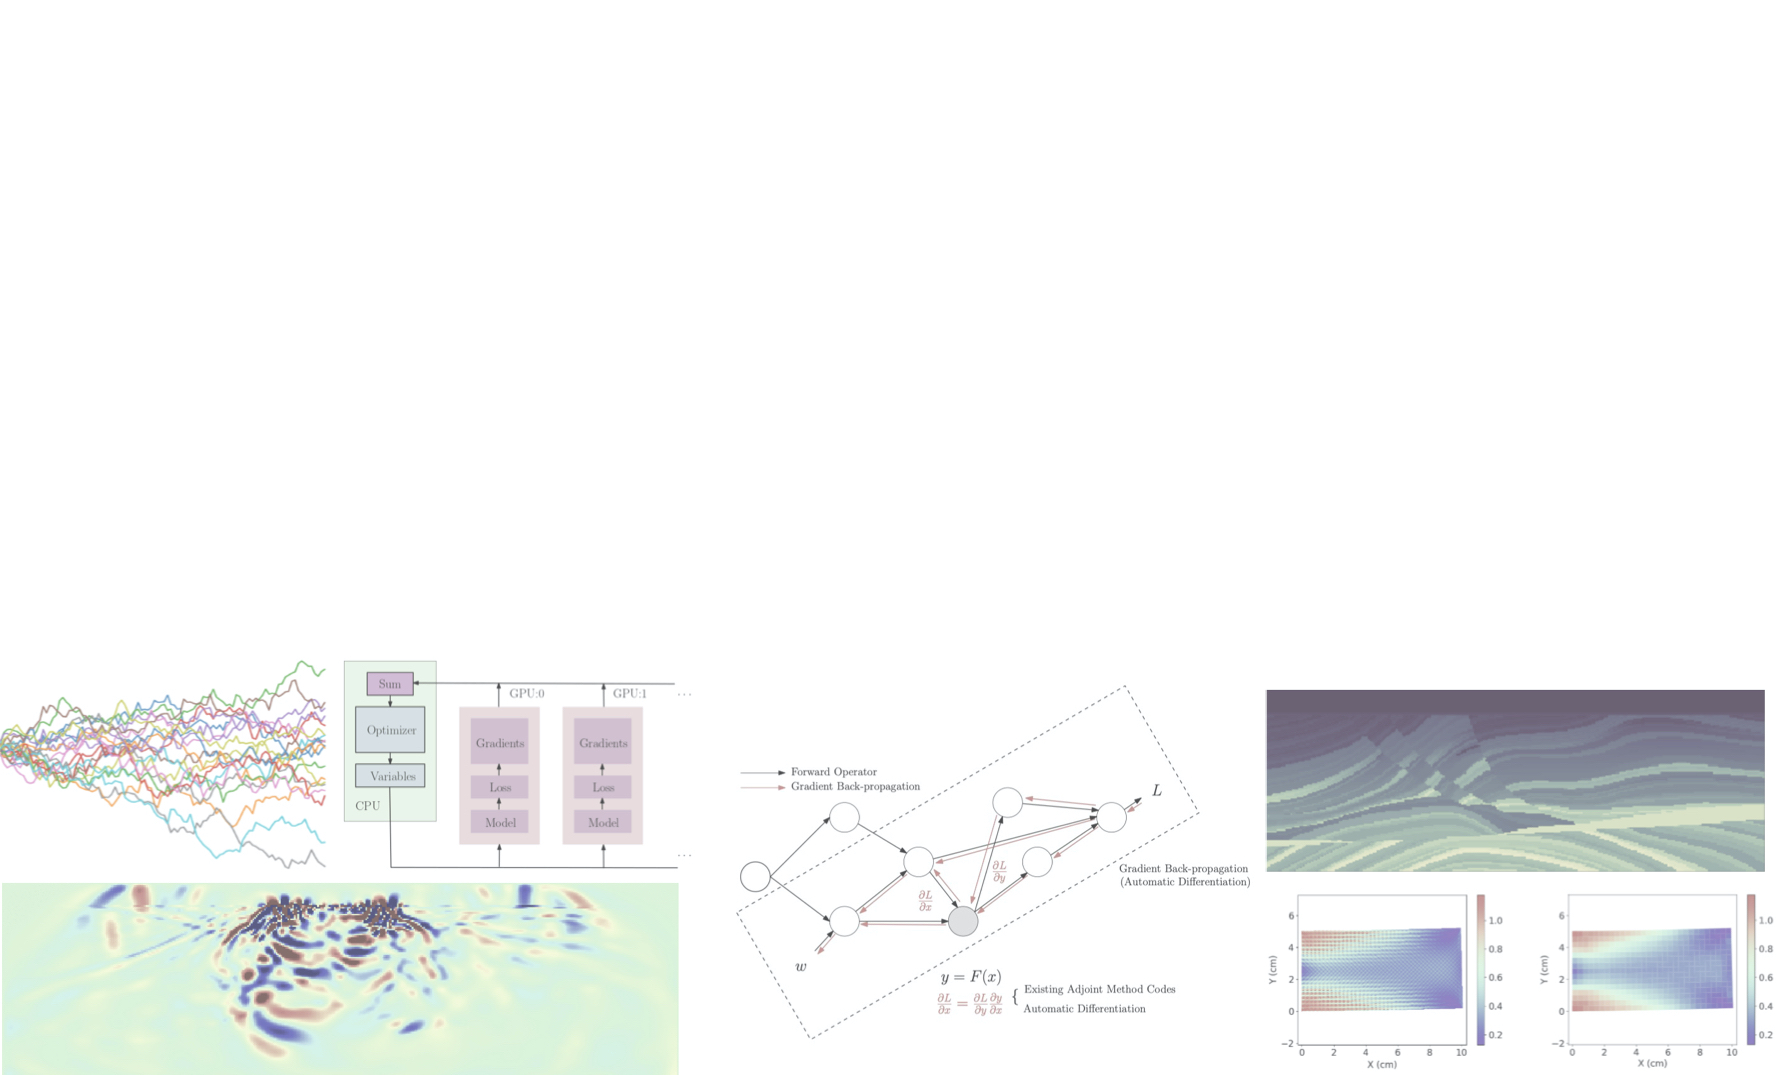
\includegraphics[width=1.0\paperwidth]{../background}}}
%\end{picture}
%  } 
%\usebackgroundtemplate{%
%  \includegraphics[width=\paperwidth,height=\paperheight]{figures/back}} 
\begin{frame}

\titlepage % Print the title page as the first slide

%dfa
\end{frame}
%\usebackgroundtemplate{}

\section{Overview}

\begin{frame}
	\frametitle{Overview}
	
	\begin{itemize}
		\item Gradients are useful in many applications
	\begin{itemize}
	\item \red{Mathematical Optimization}
		$$\min_{x\in\RR^n} \; f(x)$$
Using the gradient descent method:
$$x_{n+1} = x_n - \alpha_n \nabla f(x_n)$$
	\item \red{Sensitivity Analysis}
	$$f(x+\Delta x) \approx f'(x) \Delta x$$
	\item  \red{Machine Learning}
	
	 Training a neural network using automatic differentiation (back-propagation).
	\item \red{Solving Nonlinear Equations} Solve a nonlinear equation $f(x) = 0$ using Newton's method
	$$x_{n+1} = x_n - \frac{f(x_n)}{f'(x_n)}$$
	\end{itemize}
	
	\end{itemize}
\end{frame}


\begin{frame}
	\frametitle{Terminology}
	
	\begin{itemize}
	
	\item Deriving and implementing gradients are a challenging and all-consuming process. 
	
		\item Automatic differentiation: \red{a set of techniques to numerically evaluate the derivative of a function specified by a computer program} (Wikipedia). It also bears other names such as \red{autodiff}, \red{algorithmic differentiation}, \red{computational differentiation}, and \red{back-propagation}. 


		\item There are a lot of AD softwares
		\begin{enumerate}
			\item TensorFlow and PyTorch: deep learning frameworks in Python
			\item Adept-2: combined array and automatic differentiation library in \texttt{C++} 
			\item autograd: efficiently derivatives computation of NumPy code.
			\item ForwardDiff.jl, Zygote.jl: Julia differentiable programming packages
		\end{enumerate}
		
		 
		\item This lecture: how to compute gradients using automatic differentiation (AD)

\begin{itemize}	
	\item  Forward mode, reverse mode, and AD for implicit solvers 
	\end{itemize}
	
	
		
		 
	\end{itemize}
\end{frame}

\begin{frame}
	\frametitle{AD Software}
	
	\begin{figure}[hbt]
  \includegraphics[width=1.0\textwidth]{figures/ad_performance}
\end{figure}

{\scriptsize \url{https://github.com/microsoft/ADBench}}

\end{frame}

\begin{frame}
	\frametitle{Finite Differences}


	$$f'(x) \approx \frac{f(x+h) - f(x)}{h},\quad f'(x)\approx \frac{f(x+h) - f(x-h)}{2h}$$
	\begin{itemize}
	\item Derived from the definition of derivatives
	\begin{equation*}
		f'(x) = \lim_{h\rightarrow 0} \frac{f(x+h)-f(x)}{h}
	\end{equation*}
	\item Conceptually simple.
	\item Curse of dimensionalties: to compute the gradients of $f:\RR^m \rightarrow \RR$, you need at least $\mathcal{O}(m)$ function evaluations. 
	\item Huge numerical error: roundoff error. 
	\end{itemize}
		
\end{frame}


\begin{frame}
	\frametitle{Finite Difference}
\begin{equation*}
	f(x) = \sin(x) \quad f'(x) = \cos(x) \quad  x_0 = 0.1
\end{equation*}
	\begin{figure}[hbt]
	\centering
  \includegraphics[width=0.8\textwidth]{figures/roundoff}
\end{figure}

\end{frame}

\begin{frame}
	\frametitle{Finite Difference}
	\begin{figure}[hbt]
	\centering
  \includegraphics[width=0.8\textwidth]{figures/fd_error}
\end{figure}
\vspace{-0.5cm}
\scriptsize{Baydin, A. G., Pearlmutter, B. A., Radul, A. A., \& Siskind, J. M. (2017). Automatic differentiation in machine learning: a survey. The Journal of Machine Learning Research, 18(1), 5595-5637.}
\end{frame}

\begin{frame}
	\frametitle{Symbolic Differentiation }
		
	\begin{itemize}
		\item Symbolic differentiation computes exact derivatives (gradients): there is no approximation error. 
		\item It works by recursively applies simple rules to \textcolor{red}{symbols}
		\begin{align*}
			\frac{d}{dx}(c) &= 0  & \frac{d}{dx}(x) &= 1\\
			\frac{d}{dx}(u+v) &= \frac{d}{dx}(u) + \frac{d}{dx}(v) & \frac{d}{dx}(uv) &= v\frac{d}{dx}(u)+u\frac{d}{dx}(v)\\
			\ldots
		\end{align*}
		Here $c$ is a variable independent of $x$, and $u, v$ are variables dependent on $x$. 
	
		\item There may not exist convenient expressions for the analytical gradients of some functions. For example, a blackbox function from a third-party library. 
		
	\end{itemize}
\end{frame}

\begin{frame}
\frametitle{Symbolic Differentiation}
\begin{itemize}
\item Symbolic differentiation can lead to complex and redundant expressions
\end{itemize}
	\begin{figure}[hbt]
		\centering
  \includegraphics[width=0.8\textwidth]{figures/symbolic}
\end{figure}
\end{frame}

\begin{frame}
	\frametitle{Automatic Differentiation}
	
	\begin{itemize}
		\item AD is neither finite difference nor symbolic differentiation. 
		 \item It works by recursively applies simple rules to \textcolor{red}{values}
		\begin{align*}
			\frac{d}{dx}(c) &= 0  & \frac{d}{dx}(x) &= 1\\
			\frac{d}{dx}(u+v) &= \frac{d}{dx}(u) + \frac{d}{dx}(v) & \frac{d}{dx}(uv) &= v\frac{d}{dx}(u)+u\frac{d}{dx}(v)\\
			\ldots
		\end{align*}
		Here $c$ is a variable independent of $x$, and $u, v$ are variables dependent on $x$.
		
		\item It evaluates numerically gradients of ``function units'' using symbolic differentiation, and chains the computed gradients using the chain rule
		$$\frac{df(g(x))}{dx} = f'(g(x)) g'(x)$$
		\item It is efficient (linear in the cost of computing the function itself) and numerically stable.  
	\end{itemize}
	
\end{frame}


\section{Computational Graph}

\begin{frame}
	\frametitle{Computational Graph}
	
	\begin{itemize}
	\item The ``language'' for automatic differentiation is computational graph. 
	\begin{itemize}
	\item The computational graph is a \red{directed acyclic graph (DAG)}. 
	\item Each \red{edge} represents the data: a scalar, a vector, a matrix, or a high dimensional tensor. 
	\item Each \red{node} is a function that consumes several incoming edges and outputs some values. 
	\end{itemize}
	\begin{minipage}[c]{0.45\textwidth}
		\begin{align*}
  J &= f_4(\mathbf{u}_1, \mathbf{u}_2, \mathbf{u}_3, \mathbf{u}_4), \\
  \mathbf{u}_2 &= f_1(\mathbf{u}_1, \bm {\theta}), \\
       \mathbf{u}_3 &= f_2(\mathbf{u}_2, \bm {\theta}),\\
        \mathbf{u}_4 &= f_3(\mathbf{u}_3, \bm {\theta}).
\end{align*}
	\end{minipage}~
	\begin{minipage}[c]{0.45\textwidth}
		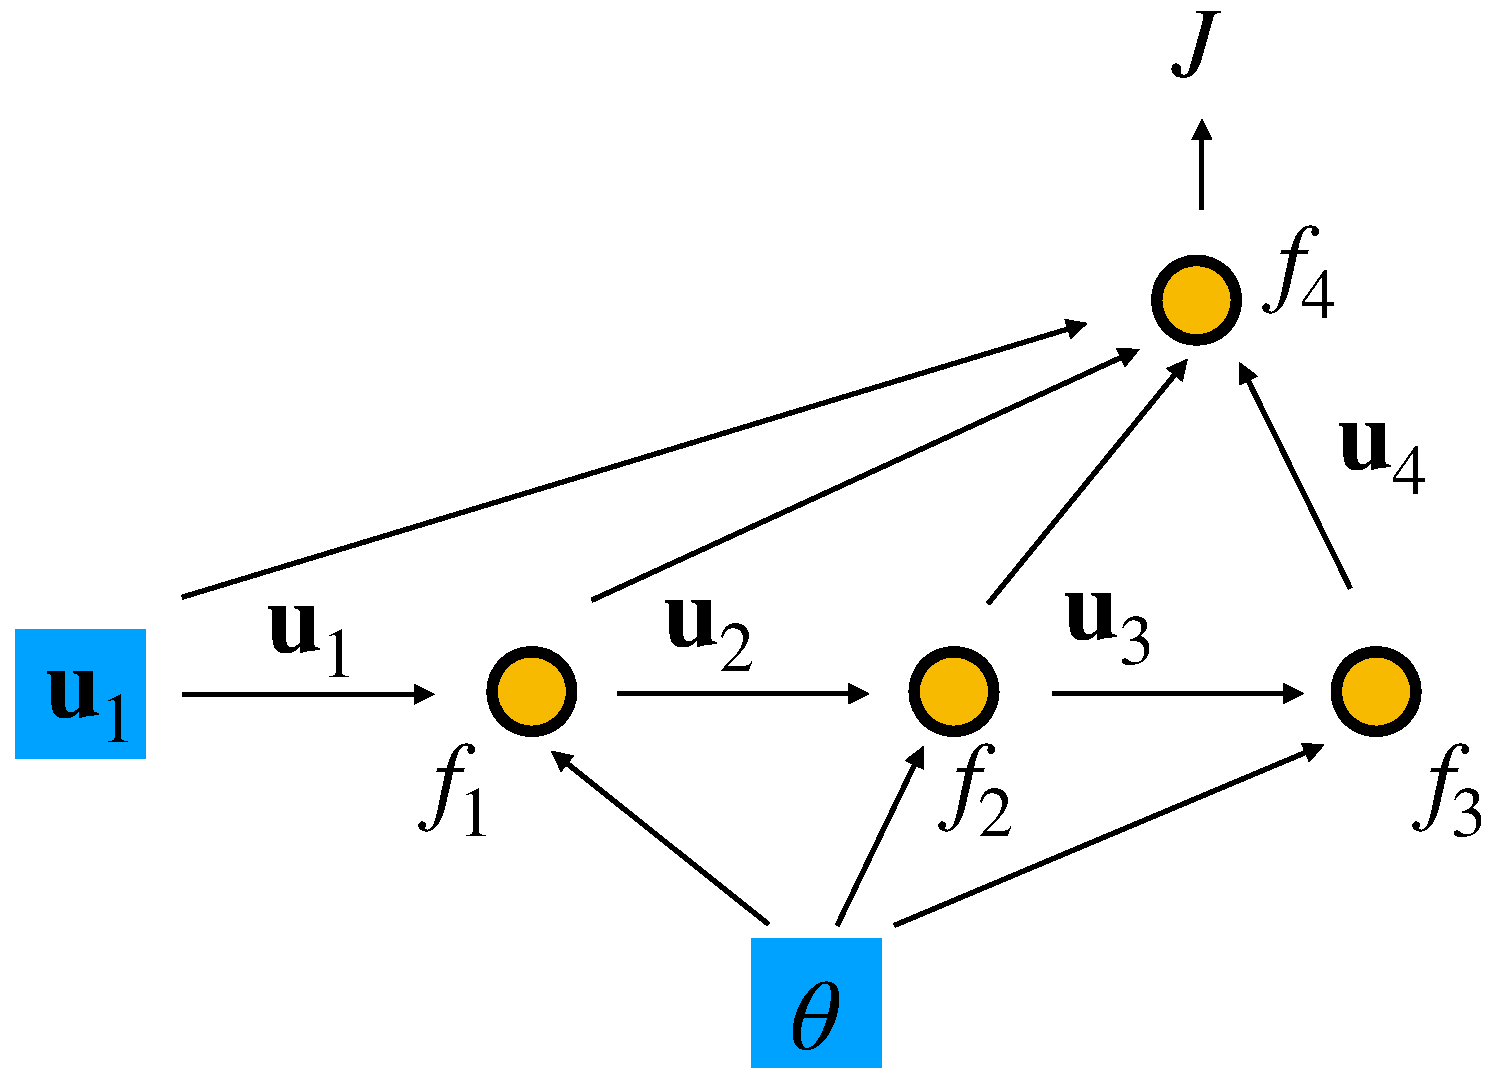
\includegraphics[width=1.0\textwidth]{../adjoint}
	\end{minipage}
	\item  Let's build a computational graph for computing 
 $$z=\sin(x_1+x_2) + x_2^2x_3$$
 
	\end{itemize}
\end{frame}


\begin{frame}
	\frametitle{Building a Computational Graph}
	
	$$z=\sin(\red{x_1+x_2}) + \red{x_2^2}x_3$$
	
	\begin{figure}[hbt]
  \includegraphics[width=0.4\textwidth]{figures/fd1}
\end{figure}

	
\end{frame}


\begin{frame}
	\frametitle{Building a Computational Graph}
	
	$$z=\red{\sin(x_1+x_2)} + \red{x_2^2x_3}$$
	
	\begin{figure}[hbt]
  \includegraphics[width=0.4\textwidth]{figures/fd2}
\end{figure}
\end{frame}

\begin{frame}
	\frametitle{Building a Computational Graph}
	
	$$z=\red{\sin(x_1+x_2) + x_2^2x_3}$$
	
	\begin{figure}[hbt]
  \includegraphics[width=0.4\textwidth]{figures/fd3}
\end{figure}
\end{frame}



\begin{frame}
	\frametitle{Computing Gradients from a Computational Graph}
	\begin{itemize}
		\item Automatic differentiation works by \textcolor{red}{propagating} gradients in the computational graph. 
		\item Two basic modes: forward-mode and backward-mode. Forward-mode propagates gradients in the same direction as forward computation. Backward-mode propagates gradients in the reverse direction of forward computation. 
		\end{itemize}
		\begin{figure}[hbt]
		\centering
  \includegraphics[width=1.0\textwidth]{figures/fb}
\end{figure}

\end{frame}


\begin{frame}
\frametitle{Computing Gradients from a Computational Graph}
	\begin{itemize}
	\item Different computational graph topologies call for different modes of automatic differentiation. 
		\begin{itemize}
		\item One-to-many: forward-propagation$\Rightarrow$forward-mode AD. 
		\begin{figure}[hbt]
  \includegraphics[width=0.6\textwidth]{figures/onetomany}
\end{figure}
		\item Many-to-one: back-propagation$\Rightarrow$reverse-mode AD.
			\end{itemize}
	\begin{figure}[hbt]
  \includegraphics[width=0.6\textwidth]{figures/manytoone}
\end{figure}
  \end{itemize} 

\end{frame}



\section{Forward Mode}



\begin{frame}
	\frametitle{Automatic Differentiation: Forward Mode AD}

	\begin{itemize}
	\item The forward-mode automatic differentiation uses the chain rule to propagate the gradients. 
	$$\frac{\partial f\circ g (x)}{\partial x} =  f'(g(x)) \red{ g'(x)}$$
		\item Compute in the same order as function evaluation. 
		\item Each node in the computational graph
		\begin{itemize}
		\item \red{Aggregate} all the gradients from up-streams. 
		\item \red{Forward} the gradient to down-stream nodes.  
		\end{itemize} 
	\end{itemize}
	
	\begin{figure}[hbt]
  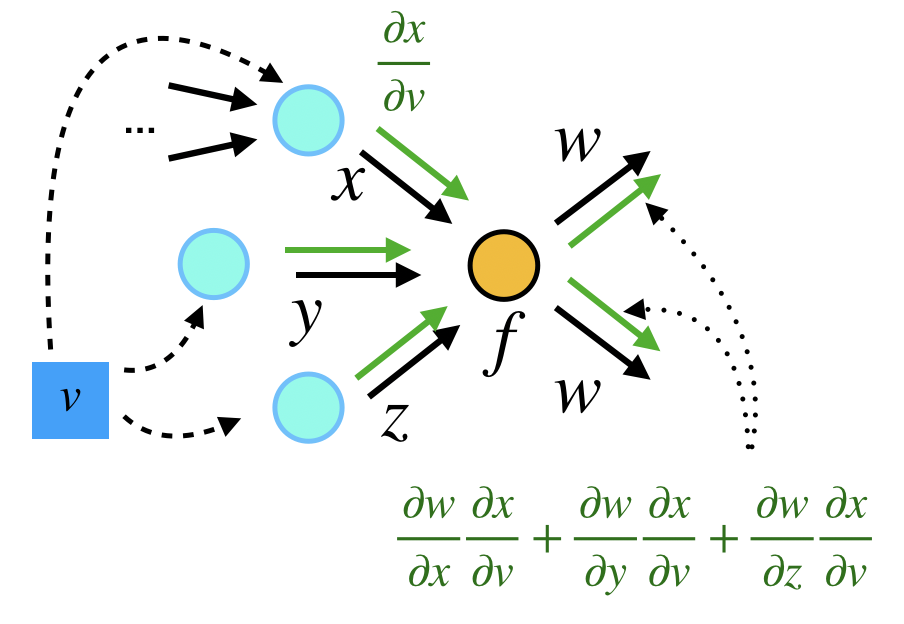
\includegraphics[width=0.4\textwidth]{../fad}
\end{figure}
	
	
\end{frame}

\begin{frame}
	\frametitle{Example: Forward Mode AD}
	\begin{itemize}
	\item 	Let's consider a specific way for computing 
	\begin{equation*}
		f(x) = \begin{bmatrix}
			x^4\\
			x^2 + \sin(x) \\
			-\sin(x)
		\end{bmatrix}
	\end{equation*}
	\end{itemize}

	
	\pause
	
	\begin{minipage}[b]{0.45\textwidth}
	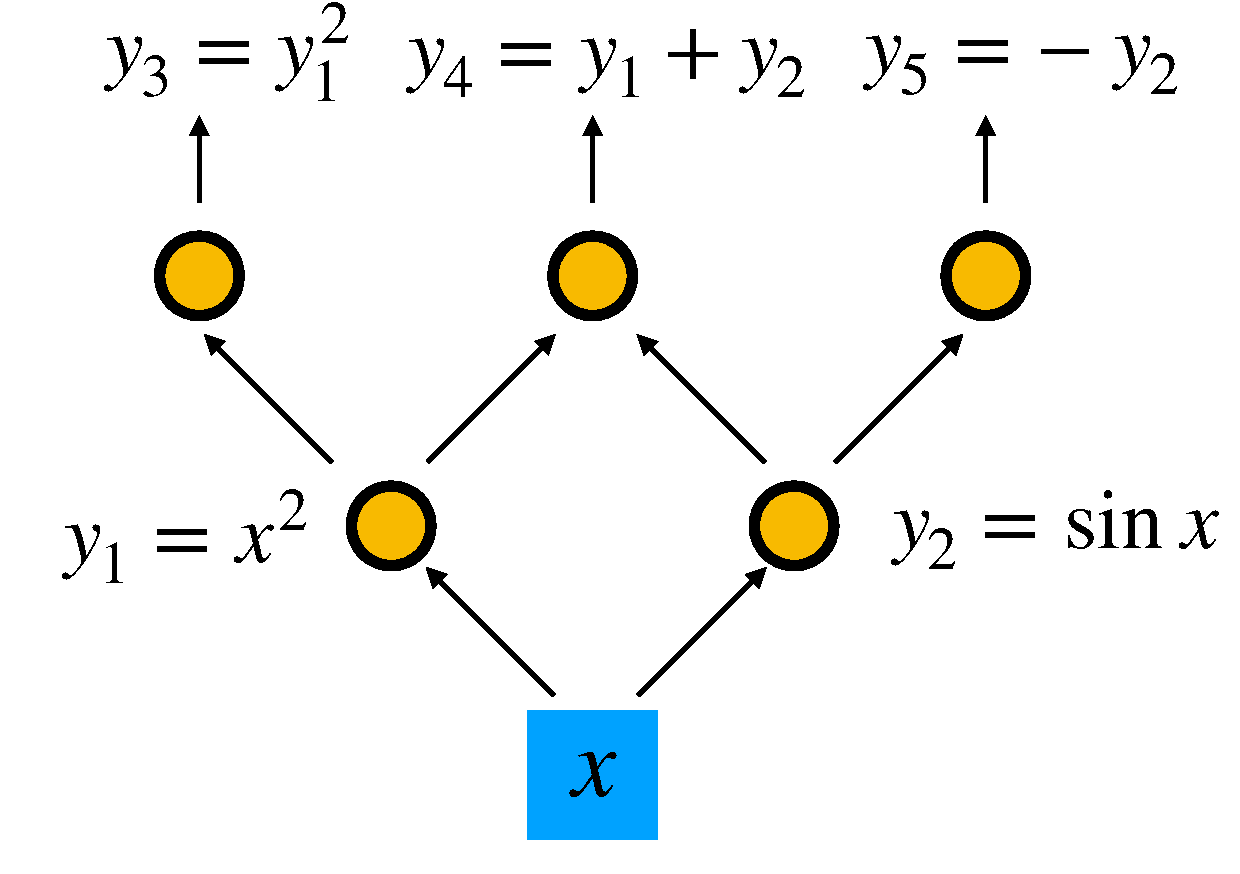
\includegraphics[width=1.0\textwidth]{../forwardmode}
\end{minipage}~
\begin{minipage}[b]{0.45\textwidth}
  \begin{align*}
\onslide<1->{(y_1, y_1')& = (x^2, 2x)} \\
\onslide<2->{(y_2, y_2') &= (\sin x, \cos x)} \\
\\
\onslide<3->{(y_3, y_3') &= (y_1^2, 2y_1y_1') = (x^4, 4x^3)}\\
 \onslide<4->{(y_4, y_4') &= (y_1+y_1, y_1'+y_2')} \\
\onslide<4->{&= (x^2+\sin x, 2x+\cos x)} \\
 \onslide<5->{(y_5, y_5')& = (-y_2, -y_2') = (-\sin x, -\cos x)}
 	\end{align*}
\end{minipage}
\end{frame}

\begin{frame}
	\frametitle{Summary}
	\begin{itemize}
		\item Forward mode AD reuses gradients from upstreams. Therefore, this mode is useful for few-to-many mappings
		$$f:\mathbb{R}^n\rightarrow \mathbb{R}^m, n\ll m$$
		\item Applications: sensitivity analysis, uncertainty quantification, etc. 
		\begin{itemize}
		\item Consider a physical model $f:\mathbb{R}^n\rightarrow \mathbb{R}^m$, let $x\in \RR^n$ be the quantity of interest (usually a low dimensional physical parameter), uncertainty propagation method computes the perturbation of the model output (usually a large dimensional quantity, i.e., $m\gg 1$)
		$$f(x+\Delta x) \approx f(x) + f'(x) \Delta x$$
		\end{itemize}
		
	\end{itemize}
\end{frame}





\section{Reverse Mode}

\begin{frame}
	\frametitle{Reverse Mode AD}
	$$\frac{df(g(x))}{dx} = \red{f'(g(x))} g'(x)$$
	\begin{itemize}
		\item Computing in the reverse order of forward computation. 
		\item Each node in the computational graph
		\begin{itemize}
		\item \red{Aggregates} all the gradients from down-streams 
		\item \red{Back-propagates} the gradient to upstream nodes.  
		\end{itemize}
		\begin{figure}[hbt]
  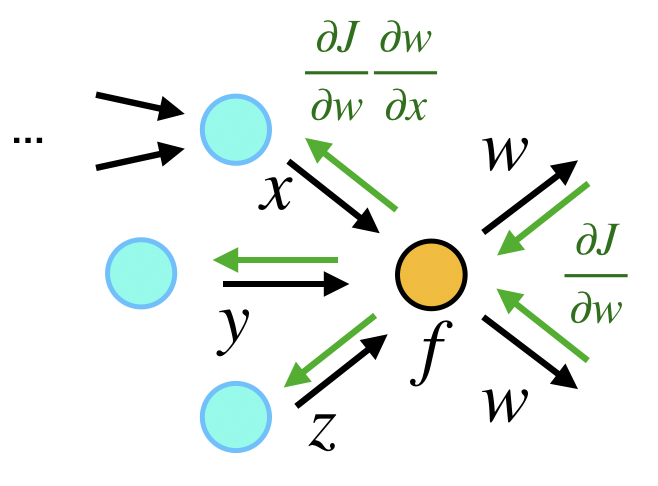
\includegraphics[width=0.4\textwidth]{../rad}
\end{figure}

	\end{itemize}
\end{frame}

\begin{frame}
\frametitle{Example: Reverse Mode AD}	
$$z=\sin(x_1+x_2) + x_2^2x_3$$
\begin{figure}[hbt]
\centering
  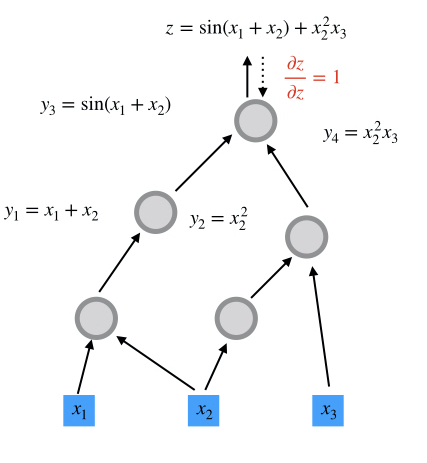
\includegraphics[width=0.5\textwidth]{figures/bd1}
\end{figure}

  
\end{frame}

\begin{frame}
\frametitle{Example: Reverse Mode AD}	
$$z=\sin(x_1+x_2) + x_2^2x_3$$
\begin{figure}[hbt]
\centering
  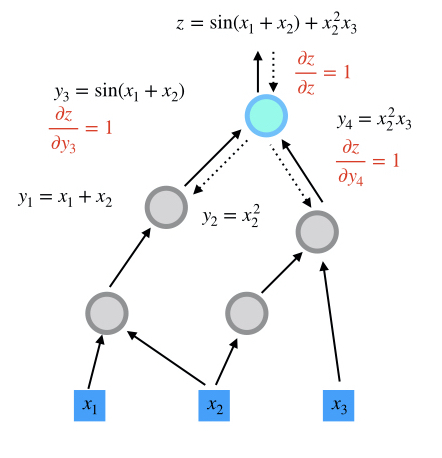
\includegraphics[width=0.5\textwidth]{figures/bd2}
\end{figure}
\end{frame}


\begin{frame}
\frametitle{Example: Reverse Mode AD}	
$$z=\sin(x_1+x_2) + x_2^2x_3$$
\begin{figure}[hbt]
\centering
  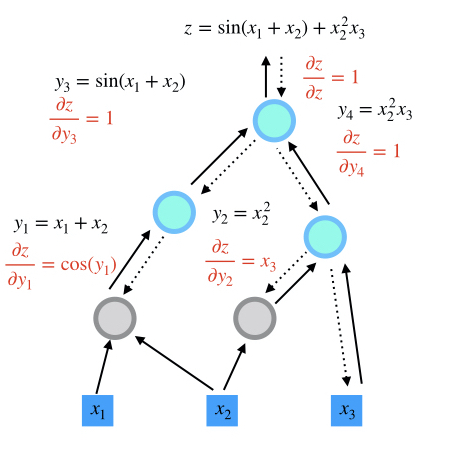
\includegraphics[width=0.5\textwidth]{figures/bd3}
\end{figure}
\end{frame}

\begin{frame}
\frametitle{Example: Reverse Mode AD}	
$$z=\sin(x_1+x_2) + x_2^2x_3$$
\begin{figure}[hbt]
\centering
  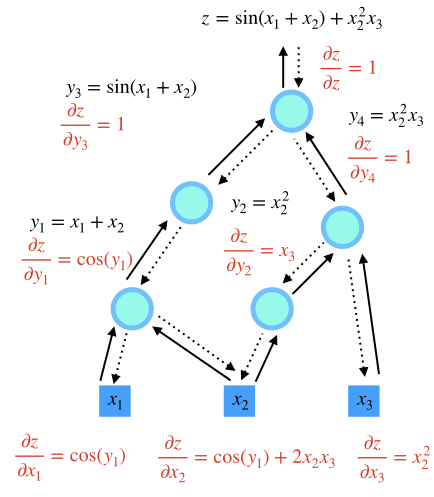
\includegraphics[width=0.5\textwidth]{figures/bd4}
\end{figure}
\end{frame}

\begin{frame}
	\frametitle{Summary}
	
	\begin{itemize}
		\item Reverse mode AD reuses gradients from down-streams. Therefore, this mode is useful for many-to-few mappings
		$$f:\mathbb{R}^n\rightarrow \mathbb{R}^m, n\gg m$$
		\item Typical application:
		\begin{itemize}
		\item Deep learning: $n=$ total number of weights and biases of the neural network, $m=1$ (loss function). 
		\item Mathematical optimization: usually there are only a single objective function. 
		\end{itemize}
	\end{itemize}
\end{frame}


\begin{frame}
	\frametitle{Summary}
	
	\begin{itemize}
		\item In general, for a function $f:\RR^n \rightarrow \RR^m$
		 % Please add the following required packages to your document preamble:
% \usepackage{booktabs}
\begin{table}[]
\centering
\begin{tabular}{@{}llll@{}}
\toprule
Mode & Suitable for ... & Complexity\footnote{$\mathrm{OPS}$ is a metric for complexity in terms of fused-multiply adds.} & Application \\ \midrule
Forward & $m\gg n$ & $\leq 2.5\;\mathrm{OPS}(f(x))$ & UQ \\
Reverse & $m\ll n$ & $\leq 4\;\mathrm{OPS}(f(x))$ & Inverse Modeling \\ \bottomrule
\end{tabular}
\end{table}
	
		
		\item There are also many other interesting topics
		\begin{itemize}
		\item Mixed mode AD: many-to-many mappings.
		\item Computing sparse Jacobian matrices using AD by exploiting sparse structures. 
		\end{itemize}
	\end{itemize}
	{\scriptsize Margossian CC. A review of automatic differentiation and its efficient implementation. Wiley Interdisciplinary Reviews: Data Mining and Knowledge Discovery. 2019 Jul;9(4):e1305.} 
\end{frame}


\section{AD for Physical Simulation}

\begin{frame}
	\frametitle{The Demand for Gradients in Physical Simulation}
	
	\begin{figure}[hbt]
  \includegraphics[width=0.9\textwidth]{figures/illu.png}
\end{figure}

	\begin{itemize}
		\item Solving nonlinear equations
		\item Uncertainty quantification/sensitivity analysis
		\item \red{Inverse problems}
	\end{itemize}
	
	\scriptsize{Image source: \url{https://mirams.wordpress.com/2016/11/23/uncertainty-in-risk-prediction/}, \url{http://fourier.eng.hmc.edu/e176/lectures/ch2/node5.html}}
\end{frame}


\begin{frame}
	\frametitle{Inverse Problem and Mathematical Optimization}
	
	\begin{itemize}
		\item Consider a bar under heating with a source term $f(x,t)$. The right hand side has fixed temperature and the left hand side is insulated. 
		\item The governing equation for the temperature $u(x,t)$ is 
		\begin{align*}
			\frac{\partial u({x}, t)}{\partial t} &= \kappa(x)\Delta u({x}, t) + f({x}, t), \quad t\in (0,T), x\in \Omega\\
			u(1, t) &= 0 \quad t>0\\
			\kappa(0)\frac{\partial u(0,t)}{\partial x} &= 0 \quad t>0
		\end{align*}
		\item The diffusivity coefficient is given by 
		$$\kappa(x) = a + bx$$
		where $a$ and $b$ are unknown parameters. 
	\end{itemize}
\end{frame}

\begin{frame}
	\frametitle{Inverse Problem and Mathematical Optimization}
	\begin{itemize}
\item Goal: calibrate $a$ and $b$ from $u_0(t) = u(0, t)$
$$\kappa(x) = a + bx$$
	\end{itemize}	
	\begin{figure}
		\centering
		\includegraphics[width=1.0\textwidth]{figures/measure}
	\end{figure}

\end{frame}
\begin{frame}
	\frametitle{Inverse Problem and Mathematical Optimization}
	\begin{itemize}
		\item This problem is a standard inverse problem. We can formulate the problem as a PDE-constrained optimization problem
		$$\begin{aligned}
\min_{a, b}\ & \int_{0}^t ( u(0, t)- u_0(t))^2 dt\\
\mathrm{s.t.}\ & \frac{\partial u(x, t)}{\partial t} = \kappa(x)\Delta u(x, t) + f(x, t), \quad t\in (0,T), x\in (0,1) \\
& -\kappa(0)\frac{\partial u(0,t)}{\partial x} = 0, t>0\\
& u(1, t) = 0, t>0\\
& u(x, 0) = 0, x\in [0,1]\\
& \kappa(x) = a x + b
\end{aligned}$$

	\end{itemize}
\end{frame}

\begin{frame}
	\frametitle{Numerical Partial Differential Equation}
	
	\begin{itemize}
		\item As with many physical modeling techniques, we discretize the PDE using numerical schemes. Here is a finite difference scheme for the PDE $k=1,2,\ldots,m, i=1,2,\ldots, n$
		$$\frac{u^{k+1}_i-u^k_i}{\Delta t} = \kappa_i \frac{u^{k+1}_{i+1}+u^{k+1}_{i-1}-2u^{k+1}_i}{\Delta x^2} + f_i^{k+1}$$
	\end{itemize}
	\begin{minipage}[c]{0.49\textwidth}
	For initial and boundary conditions, we have
		\begin{align*}
			-\kappa_1 \frac{u_2^{k}-u_0^k}{2\Delta x} &= 0\\
			u_{n+1}^k &= 0 \\
			u_i^0 &= 0
		\end{align*} 
\end{minipage}~
\begin{minipage}[c]{0.49\textwidth}
  \includegraphics[width=1.0\textwidth]{figures/grid}
\end{minipage}
	
		
\end{frame}

\begin{frame}
	\frametitle{Numerical Partial Differential Equation}
	
	\begin{itemize}
		\item Rewriting the equation as a linear system, we have
		$$A(a,b)U^{k+1} = U^k + F^{k+1}, \quad U^k = \begin{bmatrix}u_1^k\\u_2^k\\\vdots \\u_n^k\end{bmatrix}$$
		Here $\lambda_i = -\kappa_i \frac{\Delta t}{\Delta x^2}$ and 
		{\footnotesize
		\begin{equation*}
		A(a,b) = \begin{bmatrix}
2\lambda_1+1 & -2\lambda_1  &  & & \\
-\lambda_2 & 2\lambda_2+1 & -\lambda_2 & & \\
 & -\lambda_3 & 2\lambda_3 + 1 & -\lambda_3 & \\
& &\ddots & & \\
& & &\ddots & -\lambda_{n-1}\\
&&& -\lambda_n & 2\lambda_n+1
\end{bmatrix},\quad F^k = \Delta t \begin{bmatrix}
f_1^{k+1} \\
f_2^{k+1} \\
\vdots\\
f_n^{k+1}
\end{bmatrix}	
		\end{equation*}
		}
		
	\end{itemize}
\end{frame}

\begin{frame}
	\frametitle{Computational Graph for Numerical Schemes}
	
	\begin{itemize}
		\item The discretized optimization problem is 
		\begin{align*}
			\min_{a, b}& \; \sum_{k=1}^m (u^k_1 - u_0( (k-1)\Delta t))^2\\
			\text{s.t.} & \; A(a,b)U^{k+1} = U^k + F^{k+1}, k = 1, 2,\ldots, m \\
			& \; U^0 = 0
		\end{align*}
		\item The computational graph for the forward computation (evaluating the loss function) is 
		\begin{figure}[hbt]
		\centering
  \includegraphics[width=0.3\textwidth]{figures/heatcg}
\end{figure}

	\end{itemize}
\end{frame}

\begin{frame}
	\frametitle{Implementation using an AD system}
	
	\begin{figure}[hbt]
  \includegraphics[width=0.7\textwidth]{figures/simulation}
\end{figure}

\end{frame}


\section{AD Through Implicit Operators}

\begin{frame}
\frametitle{Challenges in AD}
	
	
	\begin{minipage}[t]{0.49\textwidth}
	\vspace{-3cm}
\begin{itemize}
	\item Most AD frameworks only deal with explicit operators, i.e., the functions that has analytical derivatives, or composition of these functions. 
	\item Many scientific computing algorithms are \textcolor{red}{iterative} or \textcolor{red}{implicit} in nature.
\end{itemize}
\end{minipage}~
\begin{minipage}[t]{0.49\textwidth}
  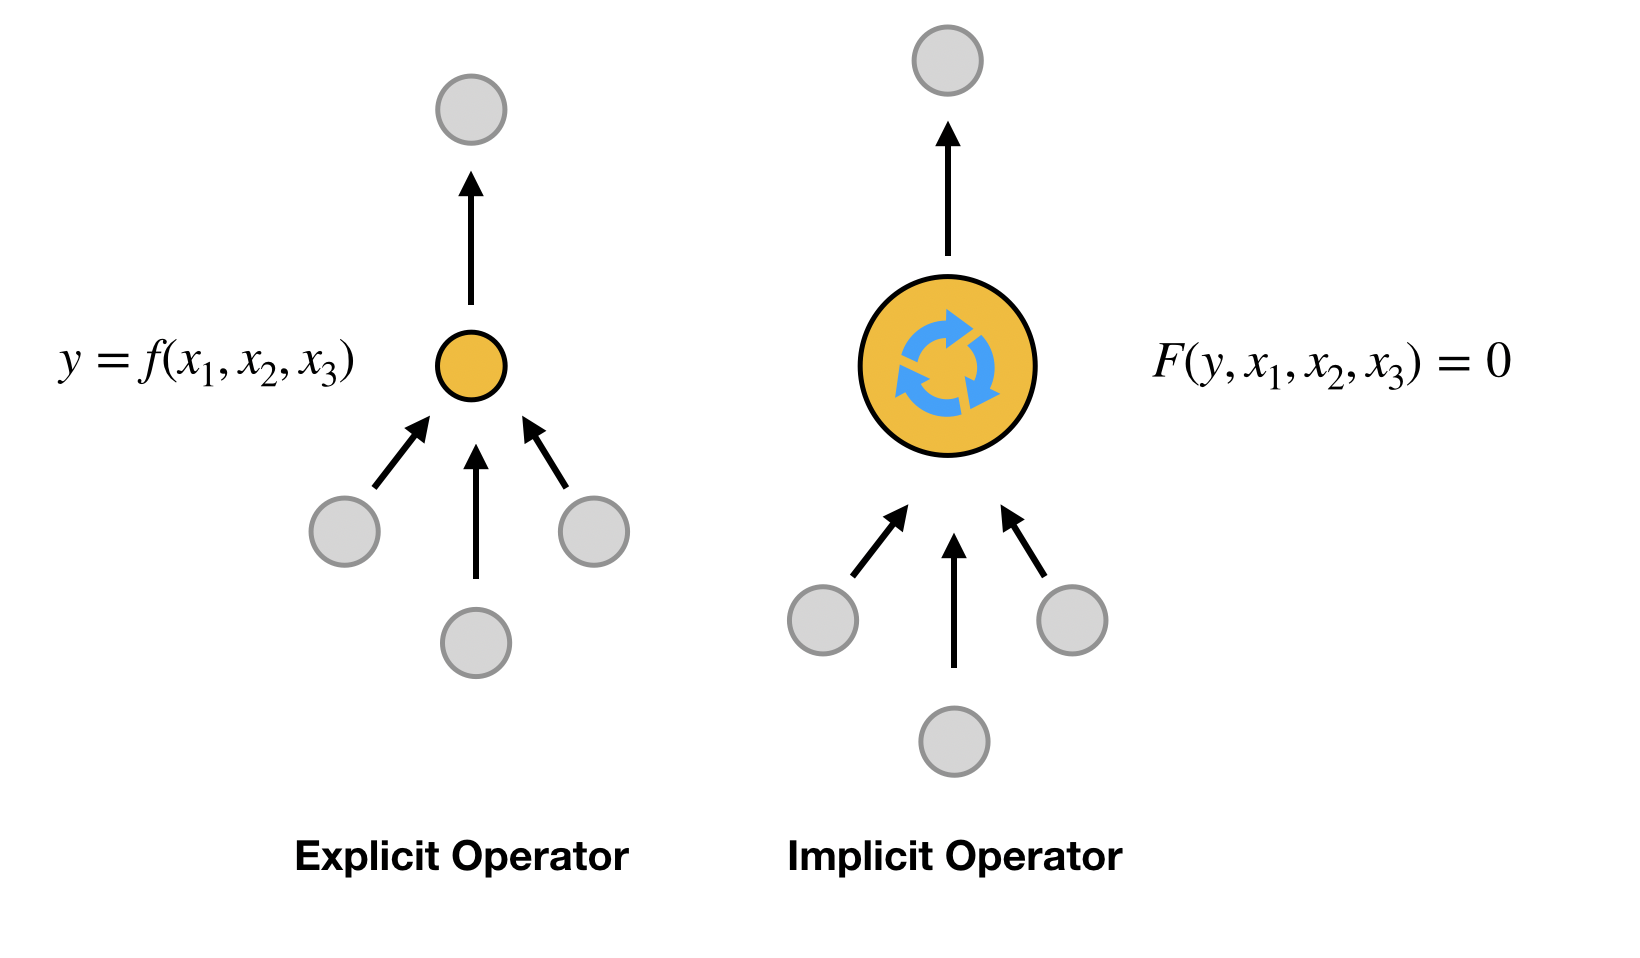
\includegraphics[width=1.0\textwidth]{../sim.png}
\end{minipage}

	% Please add the following required packages to your document preamble:
% \usepackage{booktabs}
\begin{table}[]
\begin{tabular}{@{}lll@{}}
\toprule
Linear/Nonlinear & Explicit/Implicit & Expression   \\ \midrule
Linear           & Explicit          & $y=Ax$       \\
Nonlinear        & Explicit          & $y = F(x)$   \\
\textbf{Linear}           & \textbf{Implicit}          & $Ay = x$     \\
\textbf{Nonlinear}        & \textbf{Implicit}          & $F(x,y) = 0$ \\ \bottomrule
\end{tabular}
\end{table}
\end{frame}


\begin{frame}
	\frametitle{Example}
	
\begin{itemize}
	\item Consider a function $f:x\rightarrow y$, which is implicitly defined by 
	$$F(x,y) = x^3 - (y^3+y) = 0$$
If not using the cubic formula for finding the roots, the forward computation consists of iterative algorithms, such as the Newton's method and bisection method
\end{itemize}



\begin{minipage}[t]{0.48\textwidth}
\centering
\begin{algorithmic}
\State $y^0 \gets 0$
\State $k \gets 0$
\While {$|F(x, y^k)|>\epsilon$}
\State $\delta^k \gets F(x, y^k)/F'_y(x,y^k)$
\State $y^{k+1}\gets y^k - \delta^k$
\State $k \gets k+1$
\EndWhile
\State \textbf{Return} $y^k$
\end{algorithmic}
\end{minipage}~
\begin{minipage}[t]{0.48\textwidth}
\centering
\begin{algorithmic}
\State $l \gets -M$, $r\gets M$, $m\gets 0$
\While {$|F(x, m)|>\epsilon$}
\State $c \gets \frac{a+b}{2}$
\If{$F(x, m)>0$}
\State $a\gets m$
\Else
\State $b\gets m$
\EndIf
\EndWhile
\State \textbf{Return} $c$
\end{algorithmic}

\end{minipage}	

\end{frame}

\begin{frame}
	\frametitle{Example}
	
	\begin{itemize}
		\item An efficient way is to apply the \textcolor{red}{implicit function theorem}. For our example, $F(x,y)=x^3-(y^3+y)=0$, treat $y$ as a function of $x$ and take the derivative on both sides
		$$3x^2 - 3y(x)^2y'(x)-1=0\Rightarrow y'(x) = \frac{3x^2-1}{3y(x)^2}$$
	The above gradient is \textcolor{red}{exact}.
	\end{itemize}
	
\end{frame}

\begin{frame}
	\frametitle{Implicit Operators in Physical Modeling}
	\begin{itemize}
		\item Return to our bar problem, what if the material property is complex and has a temperature-dependent governing equation?
		$$\frac{\partial u({x}, t)}{\partial t} = \red{\kappa(u)}\Delta u({x}, t) + f({x}, t), \quad t\in (0,T), x\in \Omega$$
		\item An implicit scheme is usually a nonlinear equation, and requires an iterative solver (e.g., the Newton-Raphson algorithm) to solve
		$$\frac{u^{k+1}_i-u^k_i}{\Delta t} = \red{\kappa(u_i^{k+1})} \frac{u^{k+1}_{i+1}+u^{k+1}_{i-1}-2u^{k+1}_i}{\Delta x^2} + f_i^{k+1}$$
		\item Typical AD frameworks cannot handle this operator. We need to differentiate through implicit operators. 
		\item This topic will be covered in a future lecture: \red{physics constrained learning}. 
	\end{itemize}
	
\end{frame}



\section{Conclusion}

\begin{frame}
	\frametitle{Conclusion}
	
	\begin{itemize}
		\item What's covered in this lecture
		\begin{itemize}
		\item Reverse mode automatic differentiation;
		\item Forward mode automatic differentiation;
		\item Using AD to solver inverse problems in physical modeling;
		\item Automatic differentiation through implicit operators.
		\end{itemize}
	\end{itemize}
	
\end{frame}

\begin{frame}
	\frametitle{What's Next}
	
	\begin{itemize}
	\item Physics constrained learning: inverse modeling using automatic differentiation through implicit operators;
	\item Neural networks and numerical schemes: substitute the unknown component in a physical system with a neural network and learn the neural network with AD;
	\item Implementation of inverse modeling algorithms in ADCME. 
	\end{itemize}
\end{frame}


\end{document} 